
%%%%%%%%%%%%%%%%%%%%%%%%%%%%%%%%%%%%%%%%%%%%%%%%%%%%%%%%%%%
\section{Object manipulation with hardware robots}\label{sec:realExperiment}
%%%%%%%%%%%%%%%%%%%%%%%%%%%%%%%%%%%%%%%%%%%%%%%%%%%%%%%%%%%
Our experiments use centimeter-scale hardware systems called \emph{kilobots}.  While those are far larger than the micro scale devices we model, using kilobots allows us to emulate a variety of dynamics, while enabling a high degree of control over robot function, the environment, and data collection. The kilobot is a nonholonomic, low-cost robot designed for testing collective algorithms with large numbers of robot~\cite{Rubenstein2012,rubenstein2014programmable}. It is available as an open-source platform or commercially~\cite{K-Team2015}.  Each robot is approximately 3 cm in diameter, 3 cm tall, and uses two vibration motors to move on a flat surface at speeds up to 1 cm/s.  Each robot has one ambient light sensor that is used to implement \emph{phototaxis},  moving towards a light source. 

  
\subsection{Environmental setup}  
In these experiments as shown in Fig.~\ref{fig:setup}, we used $n$=100 kilobots and a 1.5 m$\times$1.2 m whiteboard as the workspace. 
LED floodlights were placed 1.5 m above the table on the sides and corners of a square with 6 m sides. An Arduino Uno connected to an 8-relay shield controlled the lights.  

Above the table, an overhead machine vision system tracks the swarm. The vision system identifies obstacles and the object by color segmentation, determines the corners of the maze, and identifies robots using a circular Hough transform. 

\begin{figure*}
\renewcommand{\figwid}{5.25cm}
\begin{center}
	%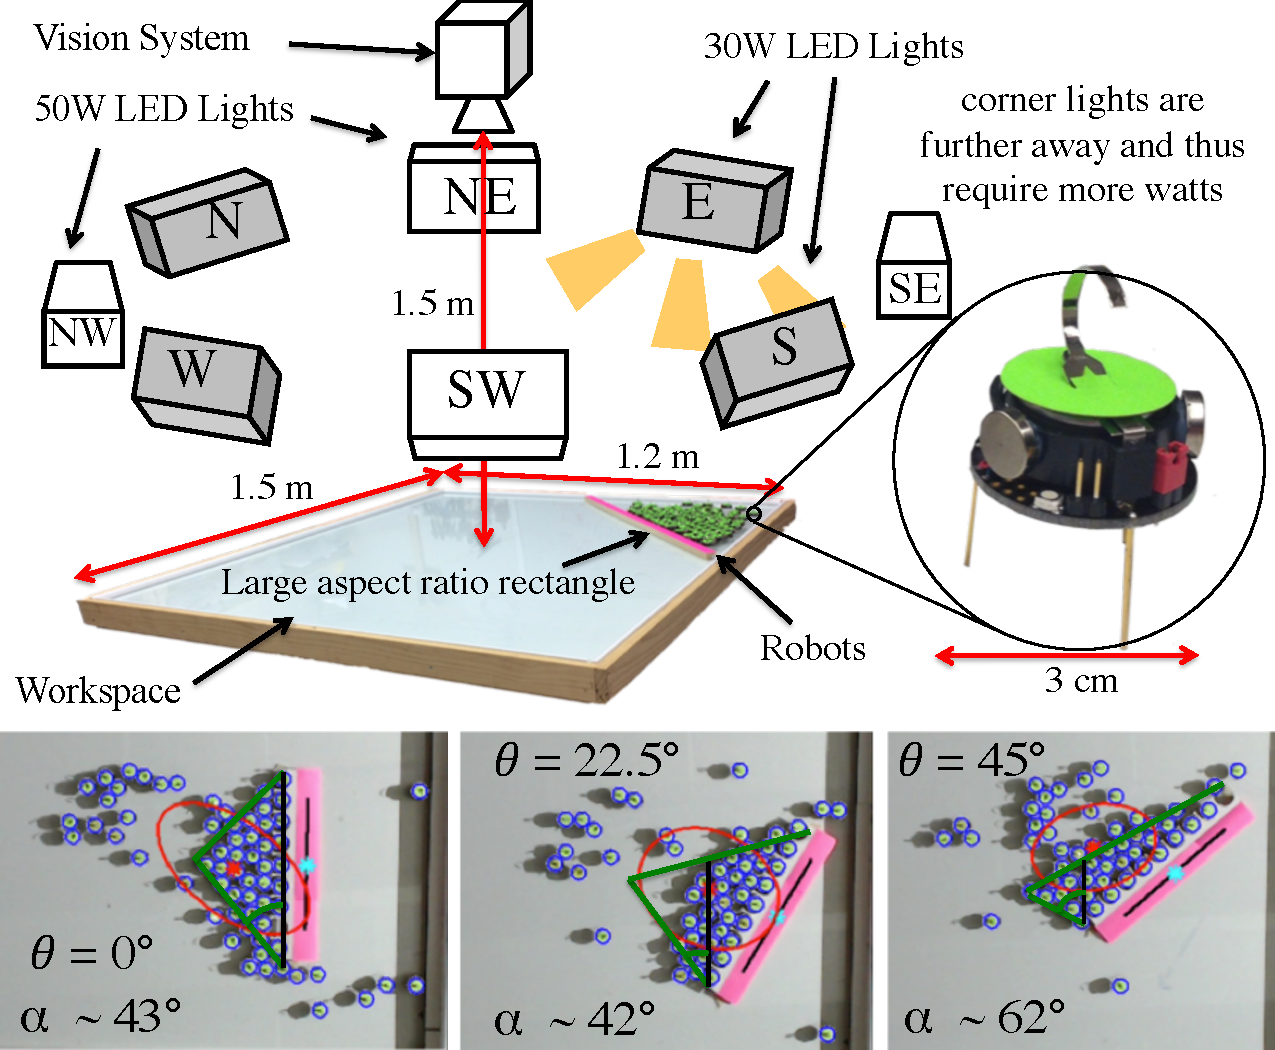
\includegraphics[width=0.5\columnwidth]{SetUp.pdf}
	\begin{overpic}[height=\figwid]{SetUp.pdf}%\put(1,75){A}
	\end{overpic}\begin{overpic}[height=5.5cm]{AllShapesR.pdf}%\put(-0,85){B}
	\end{overpic}\begin{overpic}[height=\figwid]{PotentialExp.pdf}%\put(-0,85){C}
	\end{overpic}
\end{center}
\caption{\label{fig:setup}
Hardware platform. At right are the shapes used for hardware experiments and a visualization of the potential field. }
\end{figure*}


The objects were 3D printed from ABS plastic with a paper overlay. 
Shapes included a 325 cm$^2$ equilateral triangle, 
%Small Equilateral Triangle 140 cm$^2$,
 324 cm$^2$ square,
 281 cm$^2$ hexagon,
254 cm$^2$ circle, 
and a 486 cm$^2$ %(18 cm$\times$27 cm) 
 rectangle, all shown in Fig.~\ref{fig:setup}. The laser-cut patterns for the neon green fiducial markers on the robots and 3D files for objects are available at our github repository~\cite{Shahrokhi2016blocksimulations}. 




\paragraph{Swarm mean control (hardware experiment)}

Unlike the PD controller \eqref{eq:PDcontrolPosition}, we cannot command a force input to the kilobots.  Instead, control is given by turning on one of eight lights.  The kilobots run a phototaxis routine where they search for an orientation that aligns them with the light source, and then move with an approximately constant velocity toward this light.   The kilobots oscillate along this orientation because they only have one light detector.  

We use the sign of \eqref{eq:PDcontrolPosition}, and choose the closest orientation to $\mathbf{D}(\mathbf{b})$ among the eight light sources.
Fig.~\ref{fig:realMean} shows that this limited, discretized control still enables regulating the mean position of a swarm of 100 robots.


\begin{figure}
\begin{center}
	\begin{overpic}[width=1.0\columnwidth]{RealMean}\put(6,30){\emph{t} = 90 s}\put(55,30){\emph{t} = 175 s}\end{overpic}
%	\begin{overpic}[width=0.35\columnwidth]{XYMeanControl.eps}\end{overpic}
\end{center}
\vspace{-1em}
\caption{\label{fig:realMean}
Regulating mean $x$ position of 100 kilobots using control law \eqref{eq:PDcontrolPosition}.
%Mean control plot with kilobots. %\todo{place a red star and a red circle at two spots on graph, put two images of the swar at right with a red star and red circle in left hand corner of these, and put a scale bar in image}
}
\end{figure}



\subsection{Automated object manipulation (hardware~experiment)}

Even though kilobots are nonholonomic, they performed five successful runs manipulating a hexagonal object through an obstacle maze. Videos of these runs are in Extension 2. These hardware experiments represent the results of over 100 hours of trials.
Each trial used 100 kilobots. Trials two through five were performed in a row with no failures in between.  For each trial, fully charged kilobots were placed in the lower left-hand of the workspace, as shown in Fig.~\ref{fig:expSnapShot}.  The moveable object was placed in the lower center of the workspace.  {\sc Matlab} code for vision processing, the value iteration of \S \ref{subsec:objectpolicy} and the algorithm of \S \ref{sec:AlgObjectManipulation} is available on {\sc Matlab} Central at \cite{Shahrokhi2015MDP}.
Trials were run until the object COM entered the goal region.  The trials ran for \{1465, 3457, 3000, 2162, 2707\} s.  This is $2558\pm771$ s (mean$\pm$std). 


We also tested other object shapes. 
A circular object completed in 3155 s.    
A square object completed in 6871 s. 
A rectangle and three equilateral triangle objects of varying sizes failed in a total of nine runs. 
Manipulation failures occurred when the object was pushed into a corner, requiring torque to be unstuck.  
%This paper focuses on force, but not torque control. 
Swarm torque control is the subject of our ongoing research begun in \cite{Shahrokhi2016CASE}.

%Rules: http://www.ijrr.org/historic/MMVideoGuideLines.pdf



\begin{figure}
\centering
\begin{overpic}[width=\columnwidth]{Snapshots.pdf}\put(6,80){\emph{t} = 3 s}\put(38,80){\emph{t} = 410 s}\put(70,80){\emph{t} = 710 s}
\put(15,8){\emph{t} = 1374 s}\put(48,8){\emph{t} = 2185 s}\put(80,8){\emph{t} = 2703 s}
\end{overpic}
%\vspace{-1em}
\caption{\label{fig:expSnapShot}Snapshots showing object manipulation experiment with 100 kilobots under automatic control. The automatic controller generates a policy to the goal, (see Extension 2).}
        \end{figure}



